

%\newcommand*{\ACM}{}%

\ifdefined\ACM

%\documentclass[sigplan,screen]{acmart}
\documentclass[manuscript,screen,review]{acmart}

\else
  \documentclass[18pt]{article}
\usepackage{libertine}
\usepackage{cuted}
%\usepackage{widetext}
\usepackage[utf8]{inputenc}
\usepackage[a4paper, total={6.5in, 10in} ]{geometry}
\usepackage{braket}
\usepackage{xcolor}
\usepackage{amsmath}
\usepackage{amssymb}
\usepackage{amsfonts}
\usepackage{graphicx}
\usepackage{svg}
\usepackage{float}
\usepackage{tikz}
\usetikzlibrary{patterns, shapes.arrows}
\usepackage{adjustbox}
\usepackage{tikz-network}
\usepackage[ruled,lined,linesnumbered]{algorithm2e}
\usepackage{multicol}
\usepackage[backend=biber,style=alphabetic,sorting=ynt]{biblatex}
\usepackage{xcolor}
\usepackage{pgfplots}
\DeclareUnicodeCharacter{2212}{−}
\usepgfplotslibrary{groupplots,dateplot}
\pgfplotsset{compat=newest}



\usepackage{cancel}
\usepackage{subcaption}
\addbibresource{./sample.bib}

\fi

\begin{document}
\input{newcommands}
%\title{ $\textbf{QNC}_{1} \subset $ noisy-\textbf{BQP}}
\title{ On The Cost of Fault-Tolerainzing Shallow Circuits. }
\author{Michael Ben-Or \ \ David Ponarovsky}
\maketitle

\newcommand*{\Mbas}{\mathcal{X}^\prime}
\newcommand*{\bas}{\mathcal{X}}
\newcommand*{\sMbas}{\Mbas}
\newcommand*{\QQ}{C_{X}/C_{Z}^\perp }
\newcommand*{\trig}{ Triorthogonal }
\newcommand*{\Hyp}{ Hyperproduct }
\newcommand*{\Cin}{ C_{\text{initial}} }
\newcommand*{\Ctan}{ C_{\text{Tan}} }



\newcommand*{\QACze}{ \mathbf{QAC}_{0} }
\newcommand*{\QNCzef}{ \mathbf{QNC}_{0,f} }
\newcommand*{\QNCon}{ \mathbf{QNC}_{1} }
\newcommand*{\NCon}{ \mathbf{NC}_{1} }
\newcommand*{\noiseQNCon}{ noisy-$\QNCon$ }


\abstract{In this work we study the overall depth overhead cost required for constructing fault tolerance circuits. We focus on shallow depth circuits classes, In particular, $\QACze, \QNCzef$ and $\QNCon$ and certain knowns problem candidates for demonstrating quantum advantage such as factoring \cite{Shor_1997} and Instantaneous Quantum Polynomial-time \cite{Bremner_2017}, \cite{Paletta_2024}. We only give a partial answers, Yet, clues that might pave the way towards a full understanding of the complexity versus fault tolerance trade-off. 

  \section{Introduction.} The question about the feasibility of computation under noise is almost as ancient as the computer science field itself, initialized by Von Neumann \cite{Neumann+1956+43+98} at the time that classical computation putted in debuts. Time been pass and the followed works had pointed that not even a polynomial computation in the presence of noise is still reasonable but one can implement a fault tolerance version at a most constant times cost at the circuits depth \cite{Pippenger}. Or in asymptotic sense, classical computation in the presence of noise is as exactly hard as computation in ideal environment.  

  Once again, the feasibility question raised again, this time regarding quantum computing, and while an intensive work has been done, and also succeed to prove that polynomial quantum computation can be made fault tolerance, \cite{aharonov1999faulttolerant},\cite{gottesman2014faulttolerant} and even with only constant overhead at the original circuit width \cite{grospellier:tel-03364419}, the required depth over-head is till not well understood. We stress out that in all the familiar constructions, in construct to Pippenger \cite{Pippenger}, original constant-depth gates are mapped to asymptotically grow\footnote{Note, that here, classical computation is also counted in the overall depth cost} depth gates. 
  
  This work address the above, We ask whether a magnitude depth overhead is an unavoidable price that one has to pay. And, in particular, whether an ideal $\QNCon$ circuits can be computed in noisy-$\QNCon$ circuits. We show how using the ideas presented in \cite{grospellier:tel-03364419} and \cite{Pippenger} gives almost immediately $\QNCzef \subset$ \noiseQNCon and that sampling from IQP \cite{Bremner_2017} also can be done in logarithmic depth circuits.    
  \section{ Notations. } In the following we present the notations used in the paper, readers who familiar with the literature of coding theory and quantum fault tolerance might skip \Cref{sec:classical} and \Cref{sec:quantum} and continue directly to \Cref{sec:decoders} which introduces less standard notations. 



  \begin{figure}[h]
\begin{subfigure}[h]{0.05\textwidth}
      \
    \end{subfigure}
    \begin{subfigure}[h]{0.45\textwidth}

  Once again, the feasibility question raised again, this time regarding quantum computing, and while an intensive work has been done, and also succeed to prove that polynomial quantum computation can be made fault tolerance, \cite{aharonov1999faulttolerant},\cite{gottesman2014faulttolerant} and even with only constant overhead at the original circuit width \cite{grospellier:tel-03364419}, the required depth over-head is till not well understood. We stress out that in all the familiar constructions, in construct to Pippenger \cite{Pippenger}, original constant-depth gates are mapped to asymptotically grow\footnote{Note, that here, classical computation is also counted in the overall depth cost} depth gates. 
    \end{subfigure}
    \begin{subfigure}[h]{0.05\textwidth}
      \
    \end{subfigure}
    \begin{subfigure}[h]{0.30\textwidth} 

    %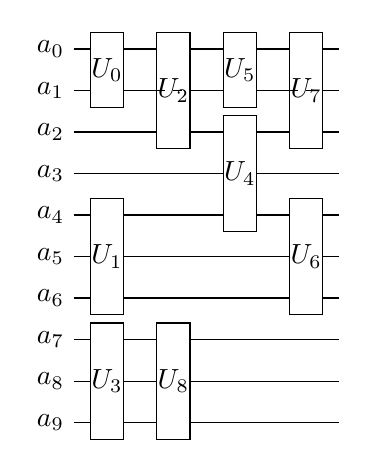
\begin{tikzpicture}[scale=1.000000,x=1pt,y=1pt]
\filldraw[color=white] (0.000000, -7.500000) rectangle (96.000000, 142.500000);
% Drawing wires
% Line 1: a0 W a_0
\draw[color=black] (0.000000,135.000000) -- (96.000000,135.000000);
\draw[color=black] (0.000000,135.000000) node[left] {$a_0$};
% Line 2: a1 W a_1
\draw[color=black] (0.000000,120.000000) -- (96.000000,120.000000);
\draw[color=black] (0.000000,120.000000) node[left] {$a_1$};
% Line 3: a2 W a_2
\draw[color=black] (0.000000,105.000000) -- (96.000000,105.000000);
\draw[color=black] (0.000000,105.000000) node[left] {$a_2$};
% Line 4: a3 W a_3
\draw[color=black] (0.000000,90.000000) -- (96.000000,90.000000);
\draw[color=black] (0.000000,90.000000) node[left] {$a_3$};
% Line 5: a4 W a_4
\draw[color=black] (0.000000,75.000000) -- (96.000000,75.000000);
\draw[color=black] (0.000000,75.000000) node[left] {$a_4$};
% Line 6: a5 W a_5
\draw[color=black] (0.000000,60.000000) -- (96.000000,60.000000);
\draw[color=black] (0.000000,60.000000) node[left] {$a_5$};
% Line 7: a6 W a_6
\draw[color=black] (0.000000,45.000000) -- (96.000000,45.000000);
\draw[color=black] (0.000000,45.000000) node[left] {$a_6$};
% Line 8: a7 W a_7
\draw[color=black] (0.000000,30.000000) -- (96.000000,30.000000);
\draw[color=black] (0.000000,30.000000) node[left] {$a_7$};
% Line 9: a8 W a_8
\draw[color=black] (0.000000,15.000000) -- (96.000000,15.000000);
\draw[color=black] (0.000000,15.000000) node[left] {$a_8$};
% Line 10: a9 W a_9
\draw[color=black] (0.000000,0.000000) -- (96.000000,0.000000);
\draw[color=black] (0.000000,0.000000) node[left] {$a_9$};
% Done with wires; drawing gates
% Line 12: a0 a1 G  $ U_{0} $
\draw (12.000000,135.000000) -- (12.000000,120.000000);
\begin{scope}
\draw[fill=white] (12.000000, 127.500000) +(-45.000000:8.485281pt and 19.091883pt) -- +(45.000000:8.485281pt and 19.091883pt) -- +(135.000000:8.485281pt and 19.091883pt) -- +(225.000000:8.485281pt and 19.091883pt) -- cycle;
\clip (12.000000, 127.500000) +(-45.000000:8.485281pt and 19.091883pt) -- +(45.000000:8.485281pt and 19.091883pt) -- +(135.000000:8.485281pt and 19.091883pt) -- +(225.000000:8.485281pt and 19.091883pt) -- cycle;
\draw (12.000000, 127.500000) node {$ U_{0} $};
\end{scope}
% Line 13: a4 a5 a6 G $ U_{1} $
\draw (12.000000,75.000000) -- (12.000000,45.000000);
\begin{scope}
\draw[fill=white] (12.000000, 60.000000) +(-45.000000:8.485281pt and 29.698485pt) -- +(45.000000:8.485281pt and 29.698485pt) -- +(135.000000:8.485281pt and 29.698485pt) -- +(225.000000:8.485281pt and 29.698485pt) -- cycle;
\clip (12.000000, 60.000000) +(-45.000000:8.485281pt and 29.698485pt) -- +(45.000000:8.485281pt and 29.698485pt) -- +(135.000000:8.485281pt and 29.698485pt) -- +(225.000000:8.485281pt and 29.698485pt) -- cycle;
\draw (12.000000, 60.000000) node {$ U_{1} $};
\end{scope}
% Line 15: a7 a8 a9 G $ U_{3} $
\draw (12.000000,30.000000) -- (12.000000,0.000000);
\begin{scope}
\draw[fill=white] (12.000000, 15.000000) +(-45.000000:8.485281pt and 29.698485pt) -- +(45.000000:8.485281pt and 29.698485pt) -- +(135.000000:8.485281pt and 29.698485pt) -- +(225.000000:8.485281pt and 29.698485pt) -- cycle;
\clip (12.000000, 15.000000) +(-45.000000:8.485281pt and 29.698485pt) -- +(45.000000:8.485281pt and 29.698485pt) -- +(135.000000:8.485281pt and 29.698485pt) -- +(225.000000:8.485281pt and 29.698485pt) -- cycle;
\draw (12.000000, 15.000000) node {$ U_{3} $};
\end{scope}
% Line 14: a0  a2  G $ U_{2} $
\draw (36.000000,135.000000) -- (36.000000,105.000000);
\begin{scope}
\draw[fill=white] (36.000000, 120.000000) +(-45.000000:8.485281pt and 29.698485pt) -- +(45.000000:8.485281pt and 29.698485pt) -- +(135.000000:8.485281pt and 29.698485pt) -- +(225.000000:8.485281pt and 29.698485pt) -- cycle;
\clip (36.000000, 120.000000) +(-45.000000:8.485281pt and 29.698485pt) -- +(45.000000:8.485281pt and 29.698485pt) -- +(135.000000:8.485281pt and 29.698485pt) -- +(225.000000:8.485281pt and 29.698485pt) -- cycle;
\draw (36.000000, 120.000000) node {$ U_{2} $};
\end{scope}
\draw[color=black,dashed] (30.000000, 120.000000) -- (42.000000, 120.000000);
% Line 20: a7 a8 a9 G $ U_{8} $
\draw (36.000000,30.000000) -- (36.000000,0.000000);
\begin{scope}
\draw[fill=white] (36.000000, 15.000000) +(-45.000000:8.485281pt and 29.698485pt) -- +(45.000000:8.485281pt and 29.698485pt) -- +(135.000000:8.485281pt and 29.698485pt) -- +(225.000000:8.485281pt and 29.698485pt) -- cycle;
\clip (36.000000, 15.000000) +(-45.000000:8.485281pt and 29.698485pt) -- +(45.000000:8.485281pt and 29.698485pt) -- +(135.000000:8.485281pt and 29.698485pt) -- +(225.000000:8.485281pt and 29.698485pt) -- cycle;
\draw (36.000000, 15.000000) node {$ U_{8} $};
\end{scope}
% Line 16: a2 a3 a4 G $ U_{4} $
\draw (60.000000,105.000000) -- (60.000000,75.000000);
\begin{scope}
\draw[fill=white] (60.000000, 90.000000) +(-45.000000:8.485281pt and 29.698485pt) -- +(45.000000:8.485281pt and 29.698485pt) -- +(135.000000:8.485281pt and 29.698485pt) -- +(225.000000:8.485281pt and 29.698485pt) -- cycle;
\clip (60.000000, 90.000000) +(-45.000000:8.485281pt and 29.698485pt) -- +(45.000000:8.485281pt and 29.698485pt) -- +(135.000000:8.485281pt and 29.698485pt) -- +(225.000000:8.485281pt and 29.698485pt) -- cycle;
\draw (60.000000, 90.000000) node {$ U_{4} $};
\end{scope}
% Line 17: a0 a1 G $ U_{5} $
\draw (60.000000,135.000000) -- (60.000000,120.000000);
\begin{scope}
\draw[fill=white] (60.000000, 127.500000) +(-45.000000:8.485281pt and 19.091883pt) -- +(45.000000:8.485281pt and 19.091883pt) -- +(135.000000:8.485281pt and 19.091883pt) -- +(225.000000:8.485281pt and 19.091883pt) -- cycle;
\clip (60.000000, 127.500000) +(-45.000000:8.485281pt and 19.091883pt) -- +(45.000000:8.485281pt and 19.091883pt) -- +(135.000000:8.485281pt and 19.091883pt) -- +(225.000000:8.485281pt and 19.091883pt) -- cycle;
\draw (60.000000, 127.500000) node {$ U_{5} $};
\end{scope}
% Line 18: a4 a5 a6 G $ U_{6} $
\draw (84.000000,75.000000) -- (84.000000,45.000000);
\begin{scope}
\draw[fill=white] (84.000000, 60.000000) +(-45.000000:8.485281pt and 29.698485pt) -- +(45.000000:8.485281pt and 29.698485pt) -- +(135.000000:8.485281pt and 29.698485pt) -- +(225.000000:8.485281pt and 29.698485pt) -- cycle;
\clip (84.000000, 60.000000) +(-45.000000:8.485281pt and 29.698485pt) -- +(45.000000:8.485281pt and 29.698485pt) -- +(135.000000:8.485281pt and 29.698485pt) -- +(225.000000:8.485281pt and 29.698485pt) -- cycle;
\draw (84.000000, 60.000000) node {$ U_{6} $};
\end{scope}
% Line 19: a0  a2  G $ U_{7} $
\draw (84.000000,135.000000) -- (84.000000,105.000000);
\begin{scope}
\draw[fill=white] (84.000000, 120.000000) +(-45.000000:8.485281pt and 29.698485pt) -- +(45.000000:8.485281pt and 29.698485pt) -- +(135.000000:8.485281pt and 29.698485pt) -- +(225.000000:8.485281pt and 29.698485pt) -- cycle;
\clip (84.000000, 120.000000) +(-45.000000:8.485281pt and 29.698485pt) -- +(45.000000:8.485281pt and 29.698485pt) -- +(135.000000:8.485281pt and 29.698485pt) -- +(225.000000:8.485281pt and 29.698485pt) -- cycle;
\draw (84.000000, 120.000000) node {$ U_{7} $};
\end{scope}
\draw[color=black,dashed] (78.000000, 120.000000) -- (90.000000, 120.000000);
% Done with gates; drawing ending labels
% Done with ending labels; drawing cut lines and comments
% Done with comments
\end{tikzpicture}

    \caption{location.}
    \label{fig:location}
    \end{subfigure} 
  \end{figure}

  \subsection{Classical and Quantum Circuits.} 
  \begin{definition}
    location $(i,j)$ of $C$. \ctt{Add here a figure of classical circuit, that demonstrates locations.}
  \end{definition}

%  \begin{figure}[h]
%    \centering
%    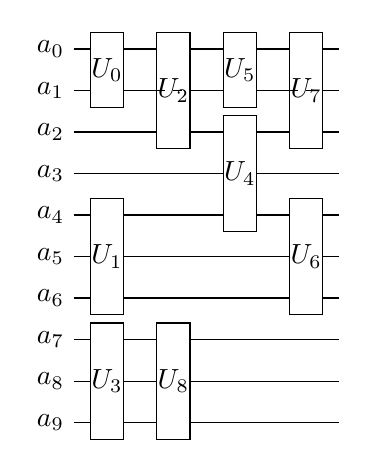
\begin{tikzpicture}[scale=1.000000,x=1pt,y=1pt]
\filldraw[color=white] (0.000000, -7.500000) rectangle (96.000000, 142.500000);
% Drawing wires
% Line 1: a0 W a_0
\draw[color=black] (0.000000,135.000000) -- (96.000000,135.000000);
\draw[color=black] (0.000000,135.000000) node[left] {$a_0$};
% Line 2: a1 W a_1
\draw[color=black] (0.000000,120.000000) -- (96.000000,120.000000);
\draw[color=black] (0.000000,120.000000) node[left] {$a_1$};
% Line 3: a2 W a_2
\draw[color=black] (0.000000,105.000000) -- (96.000000,105.000000);
\draw[color=black] (0.000000,105.000000) node[left] {$a_2$};
% Line 4: a3 W a_3
\draw[color=black] (0.000000,90.000000) -- (96.000000,90.000000);
\draw[color=black] (0.000000,90.000000) node[left] {$a_3$};
% Line 5: a4 W a_4
\draw[color=black] (0.000000,75.000000) -- (96.000000,75.000000);
\draw[color=black] (0.000000,75.000000) node[left] {$a_4$};
% Line 6: a5 W a_5
\draw[color=black] (0.000000,60.000000) -- (96.000000,60.000000);
\draw[color=black] (0.000000,60.000000) node[left] {$a_5$};
% Line 7: a6 W a_6
\draw[color=black] (0.000000,45.000000) -- (96.000000,45.000000);
\draw[color=black] (0.000000,45.000000) node[left] {$a_6$};
% Line 8: a7 W a_7
\draw[color=black] (0.000000,30.000000) -- (96.000000,30.000000);
\draw[color=black] (0.000000,30.000000) node[left] {$a_7$};
% Line 9: a8 W a_8
\draw[color=black] (0.000000,15.000000) -- (96.000000,15.000000);
\draw[color=black] (0.000000,15.000000) node[left] {$a_8$};
% Line 10: a9 W a_9
\draw[color=black] (0.000000,0.000000) -- (96.000000,0.000000);
\draw[color=black] (0.000000,0.000000) node[left] {$a_9$};
% Done with wires; drawing gates
% Line 12: a0 a1 G  $ U_{0} $
\draw (12.000000,135.000000) -- (12.000000,120.000000);
\begin{scope}
\draw[fill=white] (12.000000, 127.500000) +(-45.000000:8.485281pt and 19.091883pt) -- +(45.000000:8.485281pt and 19.091883pt) -- +(135.000000:8.485281pt and 19.091883pt) -- +(225.000000:8.485281pt and 19.091883pt) -- cycle;
\clip (12.000000, 127.500000) +(-45.000000:8.485281pt and 19.091883pt) -- +(45.000000:8.485281pt and 19.091883pt) -- +(135.000000:8.485281pt and 19.091883pt) -- +(225.000000:8.485281pt and 19.091883pt) -- cycle;
\draw (12.000000, 127.500000) node {$ U_{0} $};
\end{scope}
% Line 13: a4 a5 a6 G $ U_{1} $
\draw (12.000000,75.000000) -- (12.000000,45.000000);
\begin{scope}
\draw[fill=white] (12.000000, 60.000000) +(-45.000000:8.485281pt and 29.698485pt) -- +(45.000000:8.485281pt and 29.698485pt) -- +(135.000000:8.485281pt and 29.698485pt) -- +(225.000000:8.485281pt and 29.698485pt) -- cycle;
\clip (12.000000, 60.000000) +(-45.000000:8.485281pt and 29.698485pt) -- +(45.000000:8.485281pt and 29.698485pt) -- +(135.000000:8.485281pt and 29.698485pt) -- +(225.000000:8.485281pt and 29.698485pt) -- cycle;
\draw (12.000000, 60.000000) node {$ U_{1} $};
\end{scope}
% Line 15: a7 a8 a9 G $ U_{3} $
\draw (12.000000,30.000000) -- (12.000000,0.000000);
\begin{scope}
\draw[fill=white] (12.000000, 15.000000) +(-45.000000:8.485281pt and 29.698485pt) -- +(45.000000:8.485281pt and 29.698485pt) -- +(135.000000:8.485281pt and 29.698485pt) -- +(225.000000:8.485281pt and 29.698485pt) -- cycle;
\clip (12.000000, 15.000000) +(-45.000000:8.485281pt and 29.698485pt) -- +(45.000000:8.485281pt and 29.698485pt) -- +(135.000000:8.485281pt and 29.698485pt) -- +(225.000000:8.485281pt and 29.698485pt) -- cycle;
\draw (12.000000, 15.000000) node {$ U_{3} $};
\end{scope}
% Line 14: a0  a2  G $ U_{2} $
\draw (36.000000,135.000000) -- (36.000000,105.000000);
\begin{scope}
\draw[fill=white] (36.000000, 120.000000) +(-45.000000:8.485281pt and 29.698485pt) -- +(45.000000:8.485281pt and 29.698485pt) -- +(135.000000:8.485281pt and 29.698485pt) -- +(225.000000:8.485281pt and 29.698485pt) -- cycle;
\clip (36.000000, 120.000000) +(-45.000000:8.485281pt and 29.698485pt) -- +(45.000000:8.485281pt and 29.698485pt) -- +(135.000000:8.485281pt and 29.698485pt) -- +(225.000000:8.485281pt and 29.698485pt) -- cycle;
\draw (36.000000, 120.000000) node {$ U_{2} $};
\end{scope}
\draw[color=black,dashed] (30.000000, 120.000000) -- (42.000000, 120.000000);
% Line 20: a7 a8 a9 G $ U_{8} $
\draw (36.000000,30.000000) -- (36.000000,0.000000);
\begin{scope}
\draw[fill=white] (36.000000, 15.000000) +(-45.000000:8.485281pt and 29.698485pt) -- +(45.000000:8.485281pt and 29.698485pt) -- +(135.000000:8.485281pt and 29.698485pt) -- +(225.000000:8.485281pt and 29.698485pt) -- cycle;
\clip (36.000000, 15.000000) +(-45.000000:8.485281pt and 29.698485pt) -- +(45.000000:8.485281pt and 29.698485pt) -- +(135.000000:8.485281pt and 29.698485pt) -- +(225.000000:8.485281pt and 29.698485pt) -- cycle;
\draw (36.000000, 15.000000) node {$ U_{8} $};
\end{scope}
% Line 16: a2 a3 a4 G $ U_{4} $
\draw (60.000000,105.000000) -- (60.000000,75.000000);
\begin{scope}
\draw[fill=white] (60.000000, 90.000000) +(-45.000000:8.485281pt and 29.698485pt) -- +(45.000000:8.485281pt and 29.698485pt) -- +(135.000000:8.485281pt and 29.698485pt) -- +(225.000000:8.485281pt and 29.698485pt) -- cycle;
\clip (60.000000, 90.000000) +(-45.000000:8.485281pt and 29.698485pt) -- +(45.000000:8.485281pt and 29.698485pt) -- +(135.000000:8.485281pt and 29.698485pt) -- +(225.000000:8.485281pt and 29.698485pt) -- cycle;
\draw (60.000000, 90.000000) node {$ U_{4} $};
\end{scope}
% Line 17: a0 a1 G $ U_{5} $
\draw (60.000000,135.000000) -- (60.000000,120.000000);
\begin{scope}
\draw[fill=white] (60.000000, 127.500000) +(-45.000000:8.485281pt and 19.091883pt) -- +(45.000000:8.485281pt and 19.091883pt) -- +(135.000000:8.485281pt and 19.091883pt) -- +(225.000000:8.485281pt and 19.091883pt) -- cycle;
\clip (60.000000, 127.500000) +(-45.000000:8.485281pt and 19.091883pt) -- +(45.000000:8.485281pt and 19.091883pt) -- +(135.000000:8.485281pt and 19.091883pt) -- +(225.000000:8.485281pt and 19.091883pt) -- cycle;
\draw (60.000000, 127.500000) node {$ U_{5} $};
\end{scope}
% Line 18: a4 a5 a6 G $ U_{6} $
\draw (84.000000,75.000000) -- (84.000000,45.000000);
\begin{scope}
\draw[fill=white] (84.000000, 60.000000) +(-45.000000:8.485281pt and 29.698485pt) -- +(45.000000:8.485281pt and 29.698485pt) -- +(135.000000:8.485281pt and 29.698485pt) -- +(225.000000:8.485281pt and 29.698485pt) -- cycle;
\clip (84.000000, 60.000000) +(-45.000000:8.485281pt and 29.698485pt) -- +(45.000000:8.485281pt and 29.698485pt) -- +(135.000000:8.485281pt and 29.698485pt) -- +(225.000000:8.485281pt and 29.698485pt) -- cycle;
\draw (84.000000, 60.000000) node {$ U_{6} $};
\end{scope}
% Line 19: a0  a2  G $ U_{7} $
\draw (84.000000,135.000000) -- (84.000000,105.000000);
\begin{scope}
\draw[fill=white] (84.000000, 120.000000) +(-45.000000:8.485281pt and 29.698485pt) -- +(45.000000:8.485281pt and 29.698485pt) -- +(135.000000:8.485281pt and 29.698485pt) -- +(225.000000:8.485281pt and 29.698485pt) -- cycle;
\clip (84.000000, 120.000000) +(-45.000000:8.485281pt and 29.698485pt) -- +(45.000000:8.485281pt and 29.698485pt) -- +(135.000000:8.485281pt and 29.698485pt) -- +(225.000000:8.485281pt and 29.698485pt) -- cycle;
\draw (84.000000, 120.000000) node {$ U_{7} $};
\end{scope}
\draw[color=black,dashed] (78.000000, 120.000000) -- (90.000000, 120.000000);
% Done with gates; drawing ending labels
% Done with ending labels; drawing cut lines and comments
% Done with comments
\end{tikzpicture}

%    \caption{location.}
%    \label{fig:location}
%  \end{figure}


  \subsection{Classical Coding Theory.} \label{sec:classical} The notation used in this paper follows standard conventions for coding theory. We use $n$ to represent the length of the code, $k$ for the code's dimension, and $\rho$ for its rate. The minimum distance of the code will be denoted as $d$, and the relative distance, i.e., $d/n$, as $\delta$. In this paper, $n$ and $k$ will sometimes refer to the number of physical and logical bits. Codes will be denoted by a capital $C$ followed by either a subscript or superscript. When referring to multiple codes, we will use the above parameters as functions. For example, $\rho(C_{1})$ represents the rate of the code $C_{1}$.

Square brackets are used to present all these parameters compactly, and we use them as follows: $C=[n,k,d]$ to declare a code with the specified length, dimension, and distance. Any theorem, lemma, or claim that states a statement that is true in the asymptotic sense refers to a family of codes. The parity check matrix of the code will be denoted as $H$, with the rows of $H$ representing the parity check equations. The generator matrix of the code will be denoted as $G$, with the rows of $G$ representing the basis of codewords. The syndrome of a received word will be denoted as $s$, which is the result of multiplying $r$ by the transpose of $H$. We use $C^\perp$ to denote the dual code of $C$, which is defined such that any codeword of it $z\in C^\perp$ is orthogonal to any $x\in C$, meaning $z\cdot x = 0$, where the product is defined as $x\cdot z = \sum_{i}{x_{i}z_{i}}$. $C^{\top}$ stands for the code obtained by taking the parity check matrix of $C$ and transposing it.

In this paper, we define the triple product $\mathbb{F}_2^{n}\times \mathbb{F}_2^{n}\times\mathbb{F}_2^{n} \rightarrow \mathbb{Z}$ as $|x\cdot y \cdot z| = \sum_{i}^{n}{x_{i}y_{i}z_{i}}$. Similarly, we define the binary product $|x \cdot y|$, noting that this product differs from the standard product by mapping into $\mathbb{Z}$ rather than $\mathbb{F}_{2}$. For $w \in \mathbb{F}_{2}^{n}$, we use the super operator $ \cdot |_{w} $ to map an operator originally defined in an $n$-dimensional space to an operator that only acts on coordinates restricted to $w$. For example, $x|_{w}$ is the vector in $\mathbb{F}_{2}^{|w|}$ obtained by taking the values of $x$ on coordinates where $w$ is not zero. $|x\cdot y|_{w} = \sum_{i:w_{i}\neq 0}{x_{i}y_{i}}$ and $C|_{w}$ is the code obtained by taking the codewords of $C$ restricted to $w$.




  \subsubsection{Expander Codes}
  We saw how a graph could give us arbitrarily long codes with a positive rate. We will show, Sipser's result \cite{ExpanderCodes} that if the graph is also an expander, we can guarantee a positive relative distance. 
  \begin{definition} \label{def:mix} Denote by $\lambda$ the second eigenvalue of the adjacency matrix of the $\Delta$-regular graph. For our uses, it will be satisfied to define expander as a graph $G = \left( V,E \right)$ such that for any two subsets of vertices $T,S \subset V$, the number of edges between $S$ and $T$ is at most:
  \begin{equation*} 
    \begin{split}
      \mid E\left( S,T \right) - \frac{\Delta}{n}|S||T| \mid \le \lambda\sqrt{|S| |T|} 
    \end{split}
  \end{equation*}
\end{definition}
This bound is known as the Expander Mixining Lemma. We refer the reader to \cite{hoory2006expander} for more detailed servery. 
  \begin{theorem*} Theorem, let $C$ be the Tanner Code defined by the small code $C_{0} = [\Delta,\delta\Delta, \rho\Delta ]$ such that $\rho \ge \frac{1}{2}$ and the expander graph $G$ such that $\delta\Delta \ge \lambda$. $C$ is a good  LDPC code.
  \end{theorem*}
  \begin{proof} We have already shown that the graph has a positive rate due to the Tanner construction. So it's left to show also the code has a linear distance. Fix a codeword $x \in C$ and denote By $S$ the support of $x$ over the edges. Namely, a vertex $v\in V$ belongs to $S$ if it connects to nonzero edges regarding the assignment by $x$, Assume towards contradiction that $|x| = o\left( n \right)$. And notice that $|S|$ is at most $2|x|$, Then by The Expander Mixining Lemma we have that: 
  \begin{equation*}
    \begin{split}
      \frac{E\left( S,S \right)}{|S|} & \le \frac{\Delta}{n}|S|  + \lambda \\
      & \le_{ n \rightarrow \infty} o\left( 1 \right) + \lambda
    \end{split}
  \end{equation*}

  Namely, for any such sublinear weight string, $x$, the average of nontrivial edges for the vertex is less than $\lambda$. So there must be at least one vertex $v \in S$ that, on his local view, sets a  string at a weight less than $\lambda$. By the definition of $S$, this string cannot be trivial. Combining the fact that any nontrivial codeword of the $C_{0}$ is at weight at least $\delta\Delta$, we get a contradiction to the assumption that $v$ is satisfied, videlicet, $x$ can't be a codeword \end{proof}

  From now on, we will assume that the graphs are bipartite and we will denote the right and the left vertices by $V^{-}$ and $V^{+}$. Notice that such expanders near Ramanujan exist, see for example \cite{leverrier2022decodingquantumtannercodes}. The partition into two subsets enable us to come with a simple efficient decoder.

  Expanders code are known for having good decoders, beneath, in \Cref{alg:three}, we introduce a procedure to reduce an error. In overall, we alternately let to the right and then the left vertices to correct their own local view. In \Cref{lemma:reduce} we prove that when the applied error has size at most $\beta n$, for some constant $\beta$ then the error's weight reduced by $\frac{1}{2}$. Repeating over the procedure $\Theta(\log(n) )$ times completely correct the error. 

  We will call to the first stage, when only the right vertices suggest correction the right round, and to the second stage a left round. For the whole procedure, we will call a single correction round.  

  
  \begin{figure}[h]
    \begin{subfigure}[h]{0.05\textwidth}
      \
    \end{subfigure}
    \begin{subfigure}[h]{0.40\textwidth}

    \label{alg:three}
      \begin{algorithm}[H]
    \caption{Single decoding round}
    \KwData{ $x \in \mathbb{F}_{2}^{n}$ }
    \KwResult{ $\arg\min {\left\{  y \in C : |y + x|  \right\} }$ if $d(y,C) <$ }
    \For { $ v \in V^{+}$} {
      $x^{\prime}_{v} \leftarrow \arg\min {\left\{  y \in C_{0} : |y + x|_{v} |  \right\} } $\\
    }
    \For { $ v \in V^{-}$} {
      $x^{\prime}_{v} \leftarrow \arg\min {\left\{  y \in C_{0} : |y + x|_{v} |  \right\} } $\\
    }
    \Return  $x $

  \end{algorithm}
    \end{subfigure}
    \begin{subfigure}[h]{0.05\textwidth}
      \
    \end{subfigure}
    \begin{subfigure}[h]{0.40\textwidth} 

    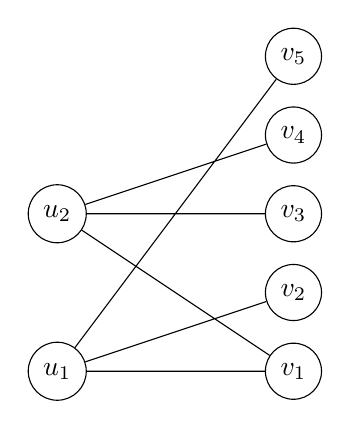
\begin{tikzpicture}%[scale=2.5]
\tikzstyle{every node}=[draw,shape=circle];

\draw node (v0) at (0,1) {$u_1$};
\draw node (v6) at (0,3) {$u_2$};
\draw node foreach \x in {1,2,3,4,5} (v\x) at (3,\x) {$v_\x$};

%\path (0:0cm) node (v0) {$v_0$};
%\path (-36:1cm) node (v1) {$v_1$};
%\path (-2*36:1cm) node (v2) {$v_2$};
%\path (0:1cm) node (v3) {$v_3$};
%\path (36:1cm) node (v4) {$v_4$};
%\path (2*36:1cm) node (v5) {$v_5$};
\draw (v0) -- (v1)
(v0) -- (v2)
(v0) -- (v5)
(v6) -- (v3)
(v6) -- (v4)
(v6) -- (v1);
\end{tikzpicture}
\caption{location.}
    \label{fig:location}
    \end{subfigure} 
  \end{figure}
  \begin{lemma}
    \label{lemma:reduce}
    If the error is at wight less than $\beta n $ then a single round of the  majority reduce the error by at least constant fraction. 
  \end{lemma}
  \begin{proof}
  Denote by $S^{(0)} \subset V^{+}$ and  $T^{(0)} \subset V^{-}$ the subsets of left and right vertices adjacent to the error. And denote by $T^{(1)} \subset T^{(0)}$ the right vertices such any of them is connect by at least $\frac{1}{2}\delta_{0}\Delta$ edges to vertices at $S^{(0))}$. Note that that any vertex in $V^{-}/T^{(1)}$ has on his local view less than $\frac{1}{2}\delta_{0}\Delta$ faulty bits, So it corrects into his right local view in the first right correction round. Therefore after the right correction round the error is set only on $T^{(1)}$'s neighbourhood, namely at size at most $\Delta|T^{(1)}|$.  We will show that this amount is strictly lower by a constant factor than $|e|$. 

  First, let's use the expansion property (\Cref{def:mix}) for getting an upper bound on $T^{(1)}$ size: \begin{equation*}
  \begin{split} 
    \frac{1}{2}\delta_{0}\Delta |T^{(1)}| & \le \Delta \frac{|T^{(1)}||S^{(0)}|}{n} + \lambda\sqrt{|T^{(1)}||S^{(0)}|} \\ 
  \left( \frac{1}{2} \delta_{0} \Delta - \frac{|S^{(0)}|}{n} \Delta \right) |T^{(1)}| & \le \lambda \sqrt{|T^{(1)}||S^{(0)}|} \\ 
|T^{(1)}| & \le \left( \frac{1}{2} \delta_{0} \Delta - \frac{|S^{(0)}|}{n} \Delta \right)^{-2}\lambda^{2} |S^{(0)}| 
  \end{split}
\end{equation*}
Since any left vertex adjoins to at most $\Delta$ faulty bits we have that $\Delta|S^{(0)}| \le |e|$. Combing with the inequality above we get:  

\begin{equation*}
  \begin{split}
    \Delta |T^{(1)}| \le \left( \frac{1}{2} \delta_{0} \Delta - \frac{|e|}{n} \right)^{-2}\lambda^{2} |e|
  \end{split}
\end{equation*}
Hence for $|e|/n \le \beta =  \frac{1}{2} \delta_{0} \Delta - \sqrt{2\lambda}$ it holds that $\Delta|T^{(1)}| \le \frac{1}{2}|e|$. Namely the error is reduced by half.  
\end{proof}

\subsubsection{Pippenger Construction.} The main insight behind Pippenger's construction is that against non trivial noise there is no point in decoding completing back to the code space since it's likely that in the follow turn the block will absorb a magnificent error. So instead of full decoding, one can perform a partial decoding round, for example, a single round of local majority. Keeping reducing the error will ensure that he distance of the state, with hight probability, will remain close (enough) to the ideal state along an ideal computation. 
 
In the original construction, any bit encoded using the repetition code, notice that the repetition code can be thought as expander code on the bipartite $\Delta$-regular graph where the local code $C_{0}$ is the repetition code on $\Delta$ bits. Then one can use \Cref{lemma:reduce} to show that a single round of decoding reduces the error by half.     

Encode any bit of the original code by $n$ bits using the repetition code. Replace any of the AND, and the OR gate by their transversal gates. In each even turn apply a single round of the majority decoder. Finally at the end apply the decoder.  


  \begin{figure}[h]
    \begin{subfigure}[h]{0.05\textwidth}
      \
    \end{subfigure}
    \begin{subfigure}[h]{0.40\textwidth}

  Once again, the feasibility question raised again, this time regarding quantum computing, and while an intensive work has been done, and also succeed to prove that polynomial quantum computation can be made fault tolerance, \cite{aharonov1999faulttolerant},\cite{gottesman2014faulttolerant} and even with only constant overhead at the original circuit width \cite{grospellier:tel-03364419}, the required depth over-head is till not well understood. We stress out that in all the familiar constructions, in construct to Pippenger \cite{Pippenger}, original constant-depth gates are mapped to asymptotically grow\footnote{Note, that here, classical computation is also counted in the overall depth cost} depth gates. 
    \end{subfigure}
    \begin{subfigure}[h]{0.05\textwidth}
      \
    \end{subfigure}
    \begin{subfigure}[h]{0.40\textwidth} 

    %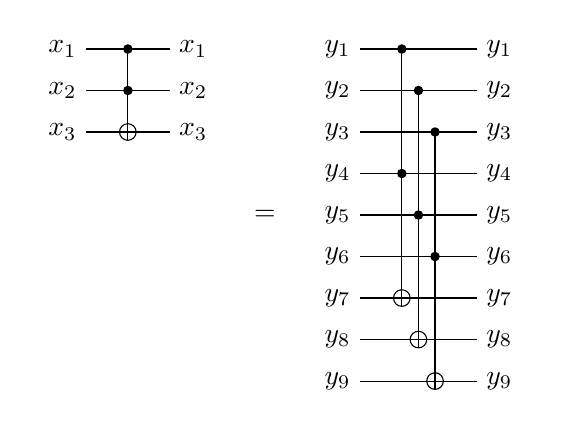
\begin{tikzpicture}[scale=1.000000,x=1pt,y=1pt]
\filldraw[color=white] (0.000000, -7.500000) rectangle (183.000000, 127.500000);
% Drawing wires
% Line 1: x_1 W x_1 x_1 y_1 y_1
\draw[color=black] (13.500000,120.000000) -- (58.500000,120.000000);
\draw[color=black] (112.500000,120.000000) -- (169.500000,120.000000);
% Line 2: x_2 W x_2 x_2 y_2 y_2
\draw[color=black] (13.500000,105.000000) -- (58.500000,105.000000);
\draw[color=black] (112.500000,105.000000) -- (169.500000,105.000000);
% Line 3: x_3 W x_3 x_3 y_3 y_3
\draw[color=black] (13.500000,90.000000) -- (58.500000,90.000000);
\draw[color=black] (112.500000,90.000000) -- (169.500000,90.000000);
% Line 7: y_4 W y_4 y_4
\draw[color=black] (112.500000,75.000000) -- (169.500000,75.000000);
% Line 8: y_5 W y_5 y_5
\draw[color=black] (112.500000,60.000000) -- (169.500000,60.000000);
% Line 9: y_6 W y_6 y_6
\draw[color=black] (112.500000,45.000000) -- (169.500000,45.000000);
% Line 10: y_7 W y_7 y_7
\draw[color=black] (112.500000,30.000000) -- (169.500000,30.000000);
% Line 11: y_8 W y_8 y_8
\draw[color=black] (112.500000,15.000000) -- (169.500000,15.000000);
% Line 12: y_9 W y_9 y_9
\draw[color=black] (112.500000,0.000000) -- (169.500000,0.000000);
% Done with wires; drawing gates
% Line 14: x_1 START
\draw[color=black] (21.000000,120.000000) node[fill=white,left,minimum height=15.000000pt,minimum width=15.000000pt,inner sep=0pt] {\phantom{$x_1$}};
\draw[color=black] (21.000000,120.000000) node[left] {$x_1$};
% Line 15: x_2 START
\draw[color=black] (21.000000,105.000000) node[fill=white,left,minimum height=15.000000pt,minimum width=15.000000pt,inner sep=0pt] {\phantom{$x_2$}};
\draw[color=black] (21.000000,105.000000) node[left] {$x_2$};
% Line 16: x_3 START
\draw[color=black] (21.000000,90.000000) node[fill=white,left,minimum height=15.000000pt,minimum width=15.000000pt,inner sep=0pt] {\phantom{$x_3$}};
\draw[color=black] (21.000000,90.000000) node[left] {$x_3$};
% Line 17: x_1 x_2 +x_3
\draw (36.000000,120.000000) -- (36.000000,90.000000);
\filldraw (36.000000, 120.000000) circle(1.500000pt);
\filldraw (36.000000, 105.000000) circle(1.500000pt);
\begin{scope}
\draw[fill=white] (36.000000, 90.000000) circle(3.000000pt);
\clip (36.000000, 90.000000) circle(3.000000pt);
\draw (33.000000, 90.000000) -- (39.000000, 90.000000);
\draw (36.000000, 87.000000) -- (36.000000, 93.000000);
\end{scope}
% Line 18: x_1 END
\draw[color=black] (51.000000,120.000000) node[fill=white,right,minimum height=15.000000pt,minimum width=15.000000pt,inner sep=0pt] {\phantom{$x_1$}};
\draw[color=black] (51.000000,120.000000) node[right] {$x_1$};
% Line 19: x_2 END
\draw[color=black] (51.000000,105.000000) node[fill=white,right,minimum height=15.000000pt,minimum width=15.000000pt,inner sep=0pt] {\phantom{$x_2$}};
\draw[color=black] (51.000000,105.000000) node[right] {$x_2$};
% Line 20: x_3 END
\draw[color=black] (51.000000,90.000000) node[fill=white,right,minimum height=15.000000pt,minimum width=15.000000pt,inner sep=0pt] {\phantom{$x_3$}};
\draw[color=black] (51.000000,90.000000) node[right] {$x_3$};
% Line 22: =
\draw[fill=white,color=white] (78.000000, -6.000000) rectangle (93.000000, 126.000000);
\draw (85.500000, 60.000000) node {$=$};
% Line 24: x_1 START
\draw[color=black] (120.000000,120.000000) node[fill=white,left,minimum height=15.000000pt,minimum width=15.000000pt,inner sep=0pt] {\phantom{$y_1$}};
\draw[color=black] (120.000000,120.000000) node[left] {$y_1$};
% Line 25: x_2 START
\draw[color=black] (120.000000,105.000000) node[fill=white,left,minimum height=15.000000pt,minimum width=15.000000pt,inner sep=0pt] {\phantom{$y_2$}};
\draw[color=black] (120.000000,105.000000) node[left] {$y_2$};
% Line 26: x_3 START
\draw[color=black] (120.000000,90.000000) node[fill=white,left,minimum height=15.000000pt,minimum width=15.000000pt,inner sep=0pt] {\phantom{$y_3$}};
\draw[color=black] (120.000000,90.000000) node[left] {$y_3$};
% Line 27: y_4 START
\draw[color=black] (120.000000,75.000000) node[fill=white,left,minimum height=15.000000pt,minimum width=15.000000pt,inner sep=0pt] {\phantom{$y_4$}};
\draw[color=black] (120.000000,75.000000) node[left] {$y_4$};
% Line 28: y_5 START
\draw[color=black] (120.000000,60.000000) node[fill=white,left,minimum height=15.000000pt,minimum width=15.000000pt,inner sep=0pt] {\phantom{$y_5$}};
\draw[color=black] (120.000000,60.000000) node[left] {$y_5$};
% Line 29: y_6 START
\draw[color=black] (120.000000,45.000000) node[fill=white,left,minimum height=15.000000pt,minimum width=15.000000pt,inner sep=0pt] {\phantom{$y_6$}};
\draw[color=black] (120.000000,45.000000) node[left] {$y_6$};
% Line 30: y_7 START
\draw[color=black] (120.000000,30.000000) node[fill=white,left,minimum height=15.000000pt,minimum width=15.000000pt,inner sep=0pt] {\phantom{$y_7$}};
\draw[color=black] (120.000000,30.000000) node[left] {$y_7$};
% Line 31: y_8 START
\draw[color=black] (120.000000,15.000000) node[fill=white,left,minimum height=15.000000pt,minimum width=15.000000pt,inner sep=0pt] {\phantom{$y_8$}};
\draw[color=black] (120.000000,15.000000) node[left] {$y_8$};
% Line 32: y_9 START
\draw[color=black] (120.000000,0.000000) node[fill=white,left,minimum height=15.000000pt,minimum width=15.000000pt,inner sep=0pt] {\phantom{$y_9$}};
\draw[color=black] (120.000000,0.000000) node[left] {$y_9$};
% Line 34: x_1 y_4 +y_7
\draw (135.000000,120.000000) -- (135.000000,30.000000);
\filldraw (135.000000, 120.000000) circle(1.500000pt);
\filldraw (135.000000, 75.000000) circle(1.500000pt);
\begin{scope}
\draw[fill=white] (135.000000, 30.000000) circle(3.000000pt);
\clip (135.000000, 30.000000) circle(3.000000pt);
\draw (132.000000, 30.000000) -- (138.000000, 30.000000);
\draw (135.000000, 27.000000) -- (135.000000, 33.000000);
\end{scope}
% Line 35: x_2 y_5 +y_8
\draw (141.000000,105.000000) -- (141.000000,15.000000);
\filldraw (141.000000, 105.000000) circle(1.500000pt);
\filldraw (141.000000, 60.000000) circle(1.500000pt);
\begin{scope}
\draw[fill=white] (141.000000, 15.000000) circle(3.000000pt);
\clip (141.000000, 15.000000) circle(3.000000pt);
\draw (138.000000, 15.000000) -- (144.000000, 15.000000);
\draw (141.000000, 12.000000) -- (141.000000, 18.000000);
\end{scope}
% Line 36: x_3 y_6 +y_9
\draw (147.000000,90.000000) -- (147.000000,0.000000);
\filldraw (147.000000, 90.000000) circle(1.500000pt);
\filldraw (147.000000, 45.000000) circle(1.500000pt);
\begin{scope}
\draw[fill=white] (147.000000, 0.000000) circle(3.000000pt);
\clip (147.000000, 0.000000) circle(3.000000pt);
\draw (144.000000, 0.000000) -- (150.000000, 0.000000);
\draw (147.000000, -3.000000) -- (147.000000, 3.000000);
\end{scope}
% Line 38: x_1 END
\draw[color=black] (162.000000,120.000000) node[fill=white,right,minimum height=15.000000pt,minimum width=15.000000pt,inner sep=0pt] {\phantom{$y_1$}};
\draw[color=black] (162.000000,120.000000) node[right] {$y_1$};
% Line 39: x_2 END
\draw[color=black] (162.000000,105.000000) node[fill=white,right,minimum height=15.000000pt,minimum width=15.000000pt,inner sep=0pt] {\phantom{$y_2$}};
\draw[color=black] (162.000000,105.000000) node[right] {$y_2$};
% Line 40: x_3 END
\draw[color=black] (162.000000,90.000000) node[fill=white,right,minimum height=15.000000pt,minimum width=15.000000pt,inner sep=0pt] {\phantom{$y_3$}};
\draw[color=black] (162.000000,90.000000) node[right] {$y_3$};
% Line 41: y_4 END
\draw[color=black] (162.000000,75.000000) node[fill=white,right,minimum height=15.000000pt,minimum width=15.000000pt,inner sep=0pt] {\phantom{$y_4$}};
\draw[color=black] (162.000000,75.000000) node[right] {$y_4$};
% Line 42: y_5 END
\draw[color=black] (162.000000,60.000000) node[fill=white,right,minimum height=15.000000pt,minimum width=15.000000pt,inner sep=0pt] {\phantom{$y_5$}};
\draw[color=black] (162.000000,60.000000) node[right] {$y_5$};
% Line 43: y_6 END
\draw[color=black] (162.000000,45.000000) node[fill=white,right,minimum height=15.000000pt,minimum width=15.000000pt,inner sep=0pt] {\phantom{$y_6$}};
\draw[color=black] (162.000000,45.000000) node[right] {$y_6$};
% Line 44: y_7 END
\draw[color=black] (162.000000,30.000000) node[fill=white,right,minimum height=15.000000pt,minimum width=15.000000pt,inner sep=0pt] {\phantom{$y_7$}};
\draw[color=black] (162.000000,30.000000) node[right] {$y_7$};
% Line 45: y_8 END
\draw[color=black] (162.000000,15.000000) node[fill=white,right,minimum height=15.000000pt,minimum width=15.000000pt,inner sep=0pt] {\phantom{$y_8$}};
\draw[color=black] (162.000000,15.000000) node[right] {$y_8$};
% Line 46: y_9 END
\draw[color=black] (162.000000,0.000000) node[fill=white,right,minimum height=15.000000pt,minimum width=15.000000pt,inner sep=0pt] {\phantom{$y_9$}};
\draw[color=black] (162.000000,0.000000) node[right] {$y_9$};
% Done with gates; drawing ending labels
% Done with ending labels; drawing cut lines and comments
% Done with comments
\end{tikzpicture}

    \caption{location.}
    \label{fig:location}
    \end{subfigure} 
  \end{figure}



%\begin{definition}
%  \label{def:trig}
%  Let $C$, $\tilde{C}$ be linear binary codes at the same length, We will say that $\tilde{C}$ is a \trig with respect to $C$ if: 
%  \begin{enumerate}
%    \item $\tilde{C} \subset C$
%    \item $|x\cdot y \cdot z|$ is even for $x,y,z \in C$ such that at least one of $x,y,z$  belongs to $\tilde{C}$. 
%    \item $|x\cdot y|$ is even for $x,y \in C$ such that at least one of $x,y$  belongs to $\tilde{C}$. 
%  \end{enumerate}
%  If a code $C$ is \trig with respect to itself then we will say that $C$ is a self \trig code. 
%\end{definition}
%For example, the empty code, that contains only the zero code word, i.e $C = \{ 0 \}$, is a \trig with respect to any code. In fact for proving \Cref{theorem:main} taking the empty code is sufficient. For other example, the \trig codes defined in \cite{bravyi2012magic} are \trig with respect to themself. 

\subsection{Quantum Codes.} \label{sec:quantum} A quantum code over $n$ qubits is an embedding of $\mathcal{H}_{2}^{\otimes k}$ as a subspace of $\mathcal{H}_{2}^{\otimes n}$. Similar to classical codes, we will call $n$ and $k$ the physical and logical qubits. The embeddings of states in $\mathcal{H}_{2}^{\otimes k}$ are called codewords or encoded states. In addition, we will use the term "logical operator" (i.e. logical $X_{i}$) to describe an operator that acts on the code space exactly as it would act on the logical space $\mathcal{H}_{2}^{\otimes k}$ (in our example, turning on and off the encoded state corresponds to the $i$th qubit exactly as $X_{i}$ acts as Pauli $X$ on the $i$th qubit in $\mathcal{H}_{2}^{\otimes k}$). 

We will denote by $X$ and $Z$ the single $X$ and $Z$ Pauli operators, by $X_{i}$ the application of $X$ on the $i$th qubit and nothing else (identity) on the rest of the qubits. By $X^{(v)}$ for some $v \in \mathbb{F}_{2}^{n}$, we mean the operator composed by applying $X$ on each of the qubits whose index is a non-trivial coordinate of $v$ and identity elsewhere. In a similar fashion, we define $Z^{(v)}$. When the context is clear, we will allow ourselves to omit the brackets, i.e. $Z^{v}$. The weight of a Pauli operator is the number of coordinates on which the operator acts non-trivially. Recall that the set of Pauli $+ I$ spans all the Hermitian matrices. We say that the Pauli weight of an operator is the maximal weight of a Pauli in its Pauli decomposition. For example, consider the operator $A = IXX + ZII$, the weight of $A$ is $2$.

The distance of a quantum code is the minimal weight of an operator that takes one codeword to another. We use the standard bracket notation to describe quantum states and in addition, we define for a vector space $A \subset \mathbb{F}_{2}^{n}$ the notation $\ket{A}$ to represent the uniform superposition of all the vectors belonging to that space, namely: \begin{equation*}
  \begin{split}
\ket{A} = \frac{1}{\sqrt{|A|}}\sum_{x \in A}{\ket{x}}
  \end{split}
\end{equation*}
We define in the same way the notation to hold for affine spaces, $\ket{x +A}$. We will use $\propto$ to denote a quantum states up to normalization factor, for example $\ket{\psi} \propto \ket{0} + \ket{1}$ means that $\ket{\psi} = \frac{1}{\sqrt{2}}(\ket{0} + \ket{1})$.
A CSS code is a quantum code defined by a pair of classical codes $C_{X}$ and $C_{Z}$, satisfying $C_{Z}^{\perp} \subset C_{X}$, such that any codeword of it has the form $\ket{x + C_{Z}^\perp}$, where $x \in C_{X}$. We will use $Q$ to refer to a CSS code in general and use $\QQ$ to refer to the vectors associated with the $X$-generators or the encoded states in the computational basis. In the same way, $C_{Z}/C_{X}^{\perp}$ refers to the $Q$ in the phase basis. We will say that a CSS code $Q$ is a LDPC if $C_{X}$ and $C_{Z}$ are both LDPC codes. Our construction uses the classical Tanner code \cite{Tanner}, the expander codes \cite{ExpanderCodes}, and \Hyp  code (quantum expanders) \cite{Leverrier_2015}, \cite{Tillich_2014}, \cite{overheadofquantumerrorcorrection}. We will not describe these constructions and refer the reader to those papers for further information.

\subsection{Decoders.} \label{sec:decoders} We denote by $C_{g}$ the good qLDPC code \cite{Dinur} \cite{Pavel} \cite{leverrier2022quantum}, and by $C_{ft}$ the concatenation code presented at \cite{aharonov1999faulttolerant} ($ft$ stands for fault tolerance). For a code $C_{y}$, we use $\Phi_{y}, E_{y}, D_{y}$ to denote the channel maps circuits into the their matched circuits compute in the code space, the encoder, and the decoder, respectively. We use $\Phi_{U}$ to denote the 'Bell'-state storing the gate $U$. We say that a state $\ket{\psi}$ is at a distance $d$ from a quantum code $C$ if there exists an operator $U$ that sends $\ket{\psi}$ into $C$ such that $U$ is spanned on Paulis with a degree of at most $d$. Sometimes, when the code being used is clear from the context, we will say that a block $B$ of qubits has absorbed at most $d$ noise if the state encoded on $B$ is at a distance of at most $d$ from that code.


\section{Todo:}
\begin{enumerate}
  \item Move to encoding each qubit by logarithmic width (instead of chanks) the reason is that the gate teleportation becomes complicated when it applied over higher dimension. 
  \item Then showing for 2-qubit gates set that is indeed works.
  \item Treating separately to noise observed in two qubits gates. 
\end{enumerate}


\section{ Fault tolerance Toffoli. } 

\ctt{In that section the $\cdot$ operation is the pair wise product (pair wise AND).}

Assume that $\bar{0}, \bar{1} \in C_{X}$ and that they belong to two different cosets of $\QQ$. Let $x,y \in \{ \bar{0},\bar{1}  \}$. 
\begin{equation}
  \label{equation:toff}
  \begin{split}
&    \sum_{z,z^{\prime},w \in \Czdu }{ \ket{z}\ket{z^{\prime}}\ket{w} } \\  
&    \sum_{z,z^{\prime},w \in \Czdu }{ \ket{z}\ket{z^{\prime}}\ket{w + z\cdot z^{\prime}} } \\  
&    \sum_{z,z^{\prime},w \in \Czdu }{ \ket{z + x }\ket{z^{\prime} + y}\ket{w + z\cdot z^{\prime}} } \\  
&    \sum_{z,z^{\prime},w \in \Czdu }{ \ket{z + x }\ket{z^{\prime} + y}\ket{ x\cdot y + x \cdot z^{\prime} + y \cdot z + z z^{\prime} + w + z\cdot z^{\prime}} } \\  
&    \sum_{z,z^{\prime},w \in \Czdu }{ \ket{z + x }\ket{z^{\prime} + y}\ket{ x\cdot y + x \cdot z^{\prime} + y \cdot z +  w } } 
  \end{split}
\end{equation}
Since $x,y \in \{ \bar{0},\bar{1}  \}$ we have that $ x\cdot z^{\prime}$ equals to either $z^{\prime}$ or $\bar{0}$. Hence $ \sum_{w \in \Czdu}{\ket { \xi +x \cdot z + w } } =  \sum_{w \in \Czdu}{\ket { \xi + w } } $. So the idea is the following, suppose that one has to compute Toffoli at time $t$ over the registers $R_{1},R_{2},R_{3}$. First, at time $0$, he initialize a logical zero $\ket{\Czdu}$ in each register, then he compute pairwise Toffoli $R_{1},R_{2}$ into $R_{3}$. That gives the ket $\sum_{z,z^{\prime},w \in \Czdu}{\ket{ z\cdot z^{\prime} + w}}$,  immediately afterwords encode $R_{3}$ again into a good quantum code. Denote by $\tau$ the time required for decoding $R_{3}$ back, at time $t-\tau$ start to decode $R_{3}$. Eventually at time time $t$ compute again the transversal Toffoli, by \Cref{equation:toff} we gets the desired.  


By similar arguments exhibited at \Cref{claim:noisepa} one can show that the errors behaves according to a Pauli noise channel. \ctt{That is not correct, since the concatenation construction assumes that all the registers initialized to physical zeros in the begging of the computation}.

\subsection{Another Idea, $z\cdot z^{\prime}$ cann't contribute too mach.}
Clearly we have that  $|z\cdot z^{\prime}| \le |z|,|z^{\prime}|$ therefore we have that $\prbm{ | z \cdot z^{\prime} | \ge t}{z,z^\prime \in \Czdu} \le \prbm{ | z | \ge t}{z\in \Czdu}$. Now assume that the tanner code by which the code defined is bipartite graph and denote by $z_{+},z_{-}$ the grouping of the $z$'s generators supported on the even and the odd vertices of the graph. By triangle inequality $|z| = |z_{+} + z_{-}| \le |z_{+}| + |z_{-}|$, So if $|z| > t$ then at least one of $|z_{-}|,|z_{+}|$ is greater than $t/2$. Hence via the union  bound: 
\begin{equation*}
  \begin{split}
    \prbm{ |z|  }{z\in \Czdu} \le \prbm{ \bigcup_{i \in \pm }{|z_{i}| \ge t/2}   }{z\in \Czdu} \le \sum_{i \in \pm }{\prbm{ |z_{i}| \ge t/2   }{z\in \Czdu}}
  \end{split}
\end{equation*}

Since any two positive (negative) generators are disjoint we have that  $|z_{+}|$ is a sum of the independent random variables each stands for the weight contributed by a positive vertex. Let us denote by $V^{+}, V^{-}$ the positive and the negative vertices and for each vertex $v \in V$ we will denote by $_{v}$ the bits of $z$ restricted to $v$ edges. So $|z_{\pm}| = \sum_{v \in V^{\pm}}{ |z_{v}| }$. For simplicity assume that $|V^{+}| = |V^{-}| = n/2$ and that $\exppm{|z|}{z \in C_{A}\otimes C_{B}} = \mu $. Then we can use concentration inequality to have: 

\begin{equation*}
  \begin{split}
    \prbm{ |z|  }{z\in \Czdu} \le \sum_{i \in \pm }{\prbm{ \sum_{v \in V^{i}}{ |z_{v}|} \ge t/2   }{z\in \Czdu}} \le 2e^{-(\mu - \frac{t}{2}) n }
  \end{split}
\end{equation*}
Thus if $\mu - \gamma  \ge O (1) $ (from \Cref{claim:error} ) then with high probability the Toffoli is computed up to reducible error.    

\subsection{Using Polynomials Codes.} Consider the CSS code above $\mathbb{F}_{q}$ defined by the stabilizers $C_{Z}^{\perp} = \braket{\{ x^{2i} : i\ge \frac{1}{2}d - c \}}$ and $C_{X}^{\perp} = \braket{\{ x^{2i+1} : i \ge \frac{1}{2}d - c \}}$ for some $c = O(1)$. Clearly the $X$-stabilizers commute with the $Z$-stabilizers. 



\section{ The Noise Model } 
Informally classical noisy circuits describe the running computation of circuits when the bits have probabilities to flip. As exactly to the classical case, in noisy quantum circuits qubits have probabilities to fault. We formalise the noise model by defining a channel $\mathcal{N} : \mathcal{C} \rightarrow \mathcal{D}\left(\mathcal{C}\right)$ that given an ideal circuit induce distribution over circuits. For example, one can consider a Pauli channel, which  after each gate of the original circuit, either do nothing with probability $1-p$ or, with probability $1-p$ impose uniformly one of the Pauli operators $X,Z,Y$. Formally:  
\begin{definition}
  Pauli channel $\mathcal{N}: \mathcal{C}\rightarrow \mathcal{D} \left( \mathcal{C} \right)$ defined to give on input $C \in \mathcal{C}$ the distribution over circuits $\tilde{C}$ where any even location of $(i, 2j)$ of $\tilde{C}$ equals to the $(i,j)$ location of $C$, and any odd location $(i,2j+1)$ of $\tilde{C}$ is the density operator $(1-p) I + \frac{p}{3} \left(X + Y + Z  \right)$. 
\end{definition}

The Pauli channel is charactered by exhibits an independent noise on the qubits, Yet for most of the fault tolerance construction a much more weaker property is required to be assumed. We say that a channel is a local stochastic noise channel if the probability to error to be occur is exponentially decays at the number of qubits the error supports.  
 
\begin{definition}
  An error channel $\mathcal{N}: \mathcal{C}\rightarrow \mathcal{D} \left( \mathcal{C} \right)$ will be said to be a local stochastic noise channel if there exists a constant $c$ such the probability to a fault to be applied on locations $(I ,j)$, where $I$ is a subset of qubits, is less than $c^{-n}$.
\end{definition}

Another important property of a noise model which we consider in this work is the accessibility to fresh qubits, also known as resets gate. When having an access to fresh qubits one can assume that in any time in the computation there are qubits at the $\ket{0}$ states. Usually those qubits are used to measured the syndrome relative to an error correction code. It was proven that without an access to fresh qubits quantum circuits cannot last than logarithmic depth without mixing into a fully mixed state, meaning to be turned into complete garbage \cite{aharonov1996limitationsnoisyreversiblecomputation}. That result also holds for a classical noisy computation. 

\begin{definition}
  An error channel $\mathcal{N}: \mathcal{C}\rightarrow \mathcal{D} \left( \mathcal{C} \right)$ will be said to has a fresh qubits access if location $(i,j)$ in an output gate $\tilde{C}$ has a non zero probability to exhibits a fault if there is a $j^{\prime} < j$ such a location $(i, j^{\prime})$ such that on the input circuit $C$, at location $(i,j^{\prime})$ a non identity gate is posed.     
\end{definition}

We close this section by formalize the \noiseQNCon class. 
\begin{definition}
  We denote by \noiseQNCon the class of decision problems solvable by logarithmic-depth quantum circuits, subjected to a local stochastic noise,  with bounded probability of error. 
\end{definition}
We mention that in \cite{aharonov1996limitationsnoisyreversiblecomputation}, it was proved how a fault tolerance circuit with an access to fresh qubits, at logarithmic depth, can be converted to a log depth circuits without a fresh qubits access at the cost which is at most polynomial in wide. Meaning that Proving that $ \QNCon \subset $ \noiseQNCon implies also that $ \QNCon $ can be computed, in the presence of noise without an access to fresh qubits. 

\section{ Fault Tolerance (With Resets gates) at Linear Depth. } 

\begin{claim}
There exists a value $p_{th} \in (0,1)$ such that if $p < p_{th}$, then any quantum circuit $C$ with a depth of $D$ and a width of $W$ can be computed by a $p$-noisy circuit $C^{\prime}$, which allows for resets. The depth of $C^{\prime}$ is at most $\max{ \{O(D), O(\log(WD)) \} }$.
\end{claim}


\subsection{Initializing Magic for Teleportation gates and encodes ancillaries.}
The Protocol: \begin{enumerate}
  \item Initialization of zeros: The qubits are divided into blocks of size $|B|$. Each block is encoded in $C_{g}$ using $D_{ft} \Phi_{ft}[E_{g}] \ket{0^{|B|}}$.
  \item Initialization of Magic for Teleportation gates: The gates in the original circuit are encoded in $C_{g}$ using $D_{ft} \Phi_{ft}[E_{g}] \ket{\Phi_{U}}$.
  \item Gate teleportation: Each gate in the original circuit is replaced by a gate teleportation.
  \item Error reduction: After the initialization step, at each time tick, each block runs a single round of error reduction.
\end{enumerate}

\begin{claim}[From \cite{leverrier2022decodingquantumtannercodes}]
  \label{claim:error} 
  Assuming that an error $|e| \le \gamma n $, i.e $e$ is supported on less than $\gamma n$ bits, then a single correction round reduce $e$ to an error $e^\prime$ such that $|e^{\prime}| < \nu |e|$. 
\end{claim}
 %Recall that by definition, $D_{i}E_{i} = I$, or in other words, $D_{i}= E_{i}^{\dagger}$.  
\begin{claim}
  \label{claim:noisepa}
  The gate $ D_{ft} \Phi_{ft}[E_{g}]$ initializes states encoded in $C_{g}$ subject to a $3p$-noise channel.  
\end{claim}
\begin{proof}
  Clearly, with high probability, $\Phi_{ft}[E_{g}]$ successfully encodes into $C_{ft} \circ C_{g}$, let's say with probability $1 - \frac{1}{poly(n)}$. Denote by $E_{i}$ and $D_{i}$ the encoder and decoder at the $i$th level of the concatenation construction. Consider the decoder under $\mathcal{N}$ action: $P_{2}D_{1}P_{2}D_{2},..,P_{i-1}D_{i}P_{i}$, by the fault-tolerance construction, a logical error at the $i$th stage occurs with probability $p^{2^{i}}$. Therefore, by the union bound, the probability that in one of the steps the circuit absorbs an error that is not corrected is less than $p + p^{2} + p^{4} + .. < 2p$. Hence, any decoded qubit absorbs noise with probability less than $2p$.


  Thus, overall, we can bound the probability of a single qubit being faulty by:
  \begin{equation*}
    \begin{split}
      \prb{\text{fault} } &=  \prb{\text{fault} |  \Phi_{ft}[E_{g}] }\cdot \prb{\Phi_{ft}[E_{g}]} + \prb{\text{fault} | \overline{\Phi_{ft}[E_{g}]} }\cdot \prb{\overline{\Phi_{ft}[E_{g}]}}\\
      &\le  \prb{\text{fault} |  \Phi_{ft}[E_{g}] } + \prb{\overline{\Phi_{ft}[E_{g}]}} \le 2p + \frac{1}{poly(n)} \le 3p
    \end{split}
  \end{equation*}

  \begin{remark}
In our construction, we use the concatenation code to encode blocks of length $\log(n)$. Therefore, any $poly(n)$ in the above should be replaced by $\log(n)$. However, this does not affect anything since the inequality does not depend on $n$.
  \end{remark}

%
%
%  \begin{equation*}
%    \begin{split}
%      \mathcal{N}(D) &= \left((\mathcal{N}(D))^{\dagger}\right)^{\dagger} =  \left(\sum_{P_{1}, P_{2}, .., P_{i} \in \mathcal{P}}{ \prb{P_{1}, P_{2}, .., P_{i}}  \left(D_{1}P_{2}D_{2},..,P_{i-1}D_{i}P_{i}\right)^{\dagger}} \right)^{\dagger} \\ 
%      &= \left( \sum_{P_{1}, P_{2}, .., P_{i} \in \mathcal{P}}{ \prb{P_{1}, P_{2}, .., P_{i}}  P_{i}E_{i}P_{i-1}E_{i-1},..,P_{1}E_{1} } \right)^{\dagger}\\
%      &= \left( \left( 1 -\frac{1}{poly(n)} \right)\sum_{P_{i} \in \mathcal{P}}\prb{P_{i}}P_{i}E + \frac{1}{poly(n)} A  \right)^{\dagger} \\ 
%      &= \left( 1 -\frac{1}{poly(n)} \right)\sum_{P_{i} \in \mathcal{P}}\prb{P_{i}}DP_{i} + \frac{1}{poly(n)} A 
%\end{split}
%  \end{equation*}
%
%  %Since $D$ is semi-transversal gate, it preserves the 
%
%
%  And notice that $\star$ is with probability $1 - \frac{1}{poly(n)}$ equals to $E_{i}E_{i-1}..,E_{1}=E$. Hence $\mathcal{N}(D)$ equals to $\left( P E \right)^{\dagger} = PD$.
%
%  \begin{equation*}
%    \begin{split}
%      \braket{ \psi^{\prime} | P_{i}E_{i}P_{i-1}E_{i-1},..,P_{1}E_{1} \psi } = \braket{ \psi^{\prime} P_{i}D_{i}P_{i-1}D_{i-1},..,P_{1}D_{1} | \psi }
%    \end{split}
%  \end{equation*}
%  Thus for any pauli-channel $\mathcal{N} : L(H) \rightarrow L(H)$, and $\psi^{\prime}$ which is a codeword we get: 
%  \begin{equation*}
%    \begin{split}
%      \braket{ \psi^{\prime} \mathcal{N}(D) | \psi } &=  \sum_{P_{1}, P_{2}, .., P_{i} \in \mathcal{P}}{ \prb{P_{1}, P_{2}, .., P_{i}}  \braket{ \psi^{\prime} P_{i}D_{i}P_{i-1}D_{i-1},..,P_{1}D_{1} | \psi }} \\
%      &=  \sum_{P_{1}, P_{2}, .., P_{i} \in \mathcal{P}^{\star}}{  \prb{P_{1}, P_{2}, .., P_{i}}\braket{ \psi^{\prime} | P_{i}E_{i}P_{i-1}E_{i-1},..,P_{1}E_{1} \psi }} \pm O(  \frac{1}{poly(n)})\\
%      &=  \sum_{P_{1}, P_{2}, .., P_{i} \in \mathcal{P}^{\star}}{  \prb{P_{1}, P_{2}, .., P_{i}}\braket{ \psi^{\prime} | P_{i} E \psi }} \pm O(  \frac{1}{poly(n)})\\
%      &\le  \sum_{ P_{i} \in \mathcal{P}}{  \prb{ P_{i}}\braket{ \psi^{\prime} | P_{i} E \psi }} \pm O(  \frac{1}{poly(n)}) \\
%      &\le  \sum_{ P_{i} \in \mathcal{P}^{\le d}}{  \prb{ P_{i}}\braket{ \psi^{\prime} | P_{i} E \psi }} \pm O (e^{-d \cdot n} ) \pm O(  \frac{1}{poly(n)}) \\
%      & \le   \sum_{ P_{i} \in \mathcal{P}/\mathcal{P}^{\star}}{  \prb{ P_{j} \in B_{d}\left( P_{i} \right)}\braket{ \psi^{\prime} | P_{i} E \psi }}  \pm O (e^{-d \cdot n} ) \pm O(  \frac{1}{poly(n)}) 
%    \end{split}
%  \end{equation*}
%  Using the fact that the concatenation code is monotonic (\Cref{def:mono}) we get that the probability to have physical fault $P_{j}$.   
%%\end{widetext}
\end{proof}

\begin{claim}
  \label{claim:prob}
  With a probability $ 1 - \frac{WD}{|B|} \cdot D 2e^{-2|B|(\beta - p)} $, the total amount of noise absorbed in a block at any given time $t$, is less than $\gamma n$. 
\end{claim}
\begin{proof}
Consider the $i$th block, denoted by $B_{i}$. By applying Hoeffding's inequality, we have that the probability that more than $\beta |B|$ qubits are flipped at time $t$ is less than $2e^{-2|B|(\beta - p)}$. By using the union bound over all blocks at all time locations, we can conclude that with probability $1 - \frac{WD}{|B|} \cdot D 2e^{-2|B|(\beta - p)}$, the noise absorbed in a block is less than $|\beta|B$ for the entire computation.

Let $X_{t}$ denote the support size of the error over $B_{i}$ at time $t$. Using \Cref{claim:error}, we can bound the total amount of error absorbed by a block until time $t$ as follows:
\begin{equation*}
\begin{split}
X_{t} \le \nu \cdot (X_{t-1} + \beta |B| ) \le \nu(\gamma+\beta) |B| \le \gamma |B|
\end{split}
\end{equation*}
\end{proof}


\begin{claim}
  The total depth of the circuit is $O ( D  ) + O ( \log^{c} |B| )$. 
\end{claim}
\begin{proof}
  The gate for encoding $|B|$-length blocks in $C_{g}$ is a Clifford gate and can therefore be computed in $O(\log|B|)$ depth. The encoding of the magic/bell states is done by first computing them in the logical space (un-encoded qubits) and then encode them using the encoder. Hence, the fault-tolerant version of both initializing ancillaries and magic states/bell states costs $O( (\log |B|) \cdot \log^{c}( |B| \log |B| ) )$ \footnote{The width of the original circuit is $|B|^{2}$ so the number of locations is $ |B|^{2} \cdot \log |B|$} depth \cite{aharonov1999faulttolerant}. Backing into $C_{g}$ from $C_{ft}$ by decoding the concatenation code takes exactly as long as the encoding, namely $O( (\log |B|) \cdot \log^{c}( |B| \log |B| ) )$.

  Then, using the bell measurements, any of the logical gates takes $O(1)$ depth. Since we only perform a single round of error correction, the remaining computation until the last decoding stage takes at most constant time of the original depth. Finally, we pay $O(\log |B|)$ for complete decoding. Summing all, we get: 
  \begin{equation*}
    \begin{split}
     &  O ( \log |B|\cdot  \log^{c}( |B| \log |B| ) )  + O ( D  ) + O ( \log |B| ) \\ 
     = & O ( D  ) + O ( \log^{c} |B| )
    \end{split}
  \end{equation*}
\end{proof}

Assuming that $W$ is polynomial in $D$, taking the block length to be $|B| = \log((W \cdot D)^c)$, as shown in \Cref{claim:prob}, results in a linear fault tolerance construction with a success probability of $1 - \frac{1}{\log^{c_2}(W \cdot D)}$. This means that the fault tolerance version of circuits in $\textbf{QNC}_1$ has a logarithmic depth. Additionally, using the construction in \cite{aharonov1996limitationsnoisyreversiblecomputation} produces a polynomial fault tolerance circuit in the reversible gates setting. \ctt{ We missed the fact that it requires non trivial classical computation to compute what gate should be applied after the gate teleportation (i.e $UPU^{\dagger}$ )}.



\section{ Does $\NCon \subset $\noiseQNCon ?}


\section{ Does Factoring $\subset$ \noiseQNCon ?}

\begin{equation*}
  \begin{split}
    D(n) &= \Theta(\log n ) + D(\sqrt{n})\\
    \Rightarrow D(n) & = \Theta( \log n ) 
  \end{split}
\end{equation*}



%\input{./tempmagic.tex}
%\cite{leverrier2022quantum}
%\cite{moore1998parallel}
%\cite{Tillich_2014}
%\cite{meier2012magicstate}
%\cite{bravyi2012magic}

\section{Overhead by Simple Counting Arguments.} 
Denote by $\Gamma(n,l)$ the number of circuits over $n$ qubits at length at most $n$. We can bound the number of noisy versions of logical circuits over $k, qubits$ as followes: 
\begin{equation*}
  \begin{split}
    \Gamma(k,l) & \cdot \left( { n \choose \Delta  } \cdot \gamma^{\Delta} \right)^{l} \le \Gamma(n,l) \\   
    \Rightarrow & 2^{  nl \left( H(\delta) +  \delta\log_{2}\gamma \right)  } \le \frac{\Gamma(n,l\cdot c)}{\Gamma(k,l)}
  \end{split}
\end{equation*}


\printbibliography


\end{document}

